\section{Pipe testing}
\textbf{Выданные параметры:} [pipe-data-size,pipe-ops]
\subsection{pipe}
\nquote{--pipe N}{start N workers that perform large pipe writes and reads to exercise pipe I/O.  This exercises memory write  and
reads as well as context switching.  Each worker has two processes, a reader and a writer.}
Найдем оптимальное количество воркеров:\\
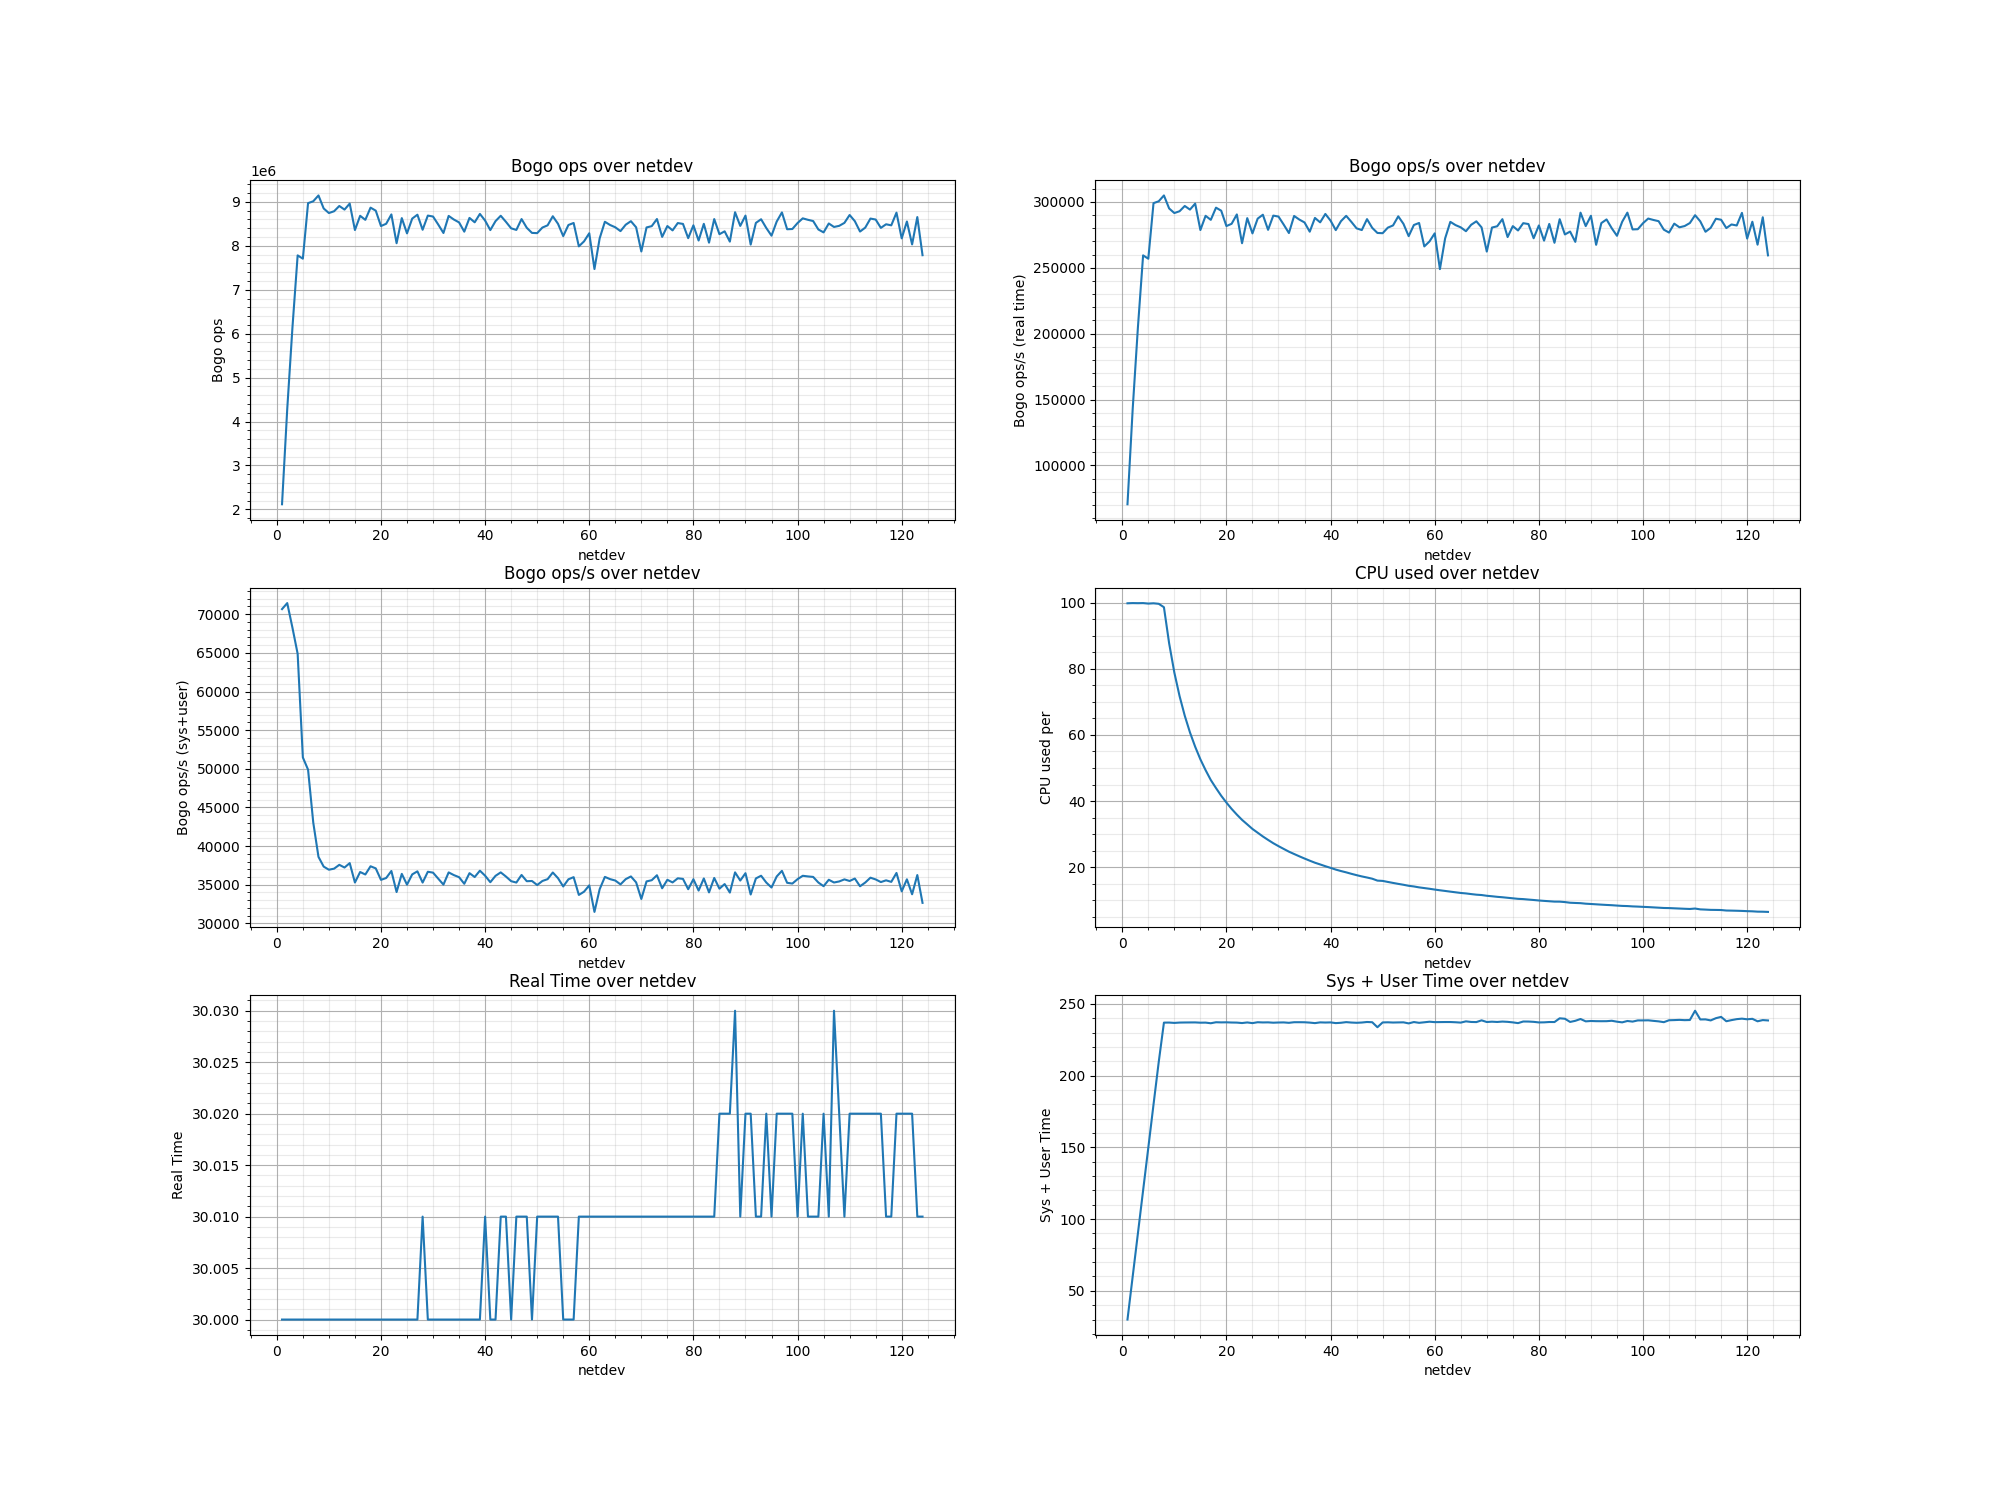
\includegraphics[width=\textwidth]{./network/image/netdev-bogops.png}
Максимум bogo ops достигается при 4.
\subsection{pipe-ops}
\nquote{--pipe-ops N}{stop pipe stress workers after N bogo pipe write operations.}
Попробуем оценить производительность по \textit{bogo ops/s}
\lstinputlisting[]{pipe/scripts/pipe-ops.zsh}
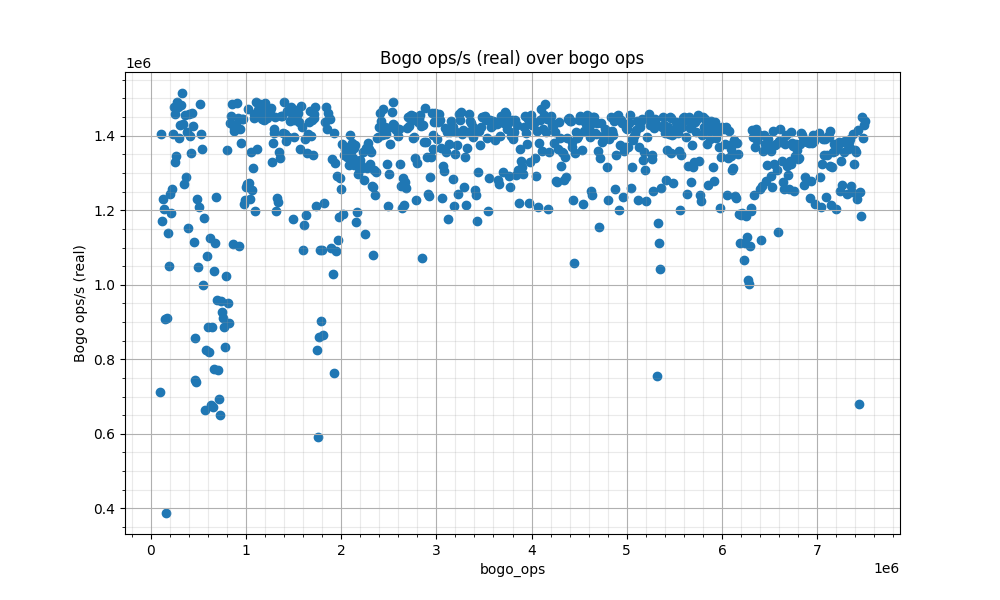
\includegraphics[width=\textwidth]{./pipe/image/pipe-ops.png}
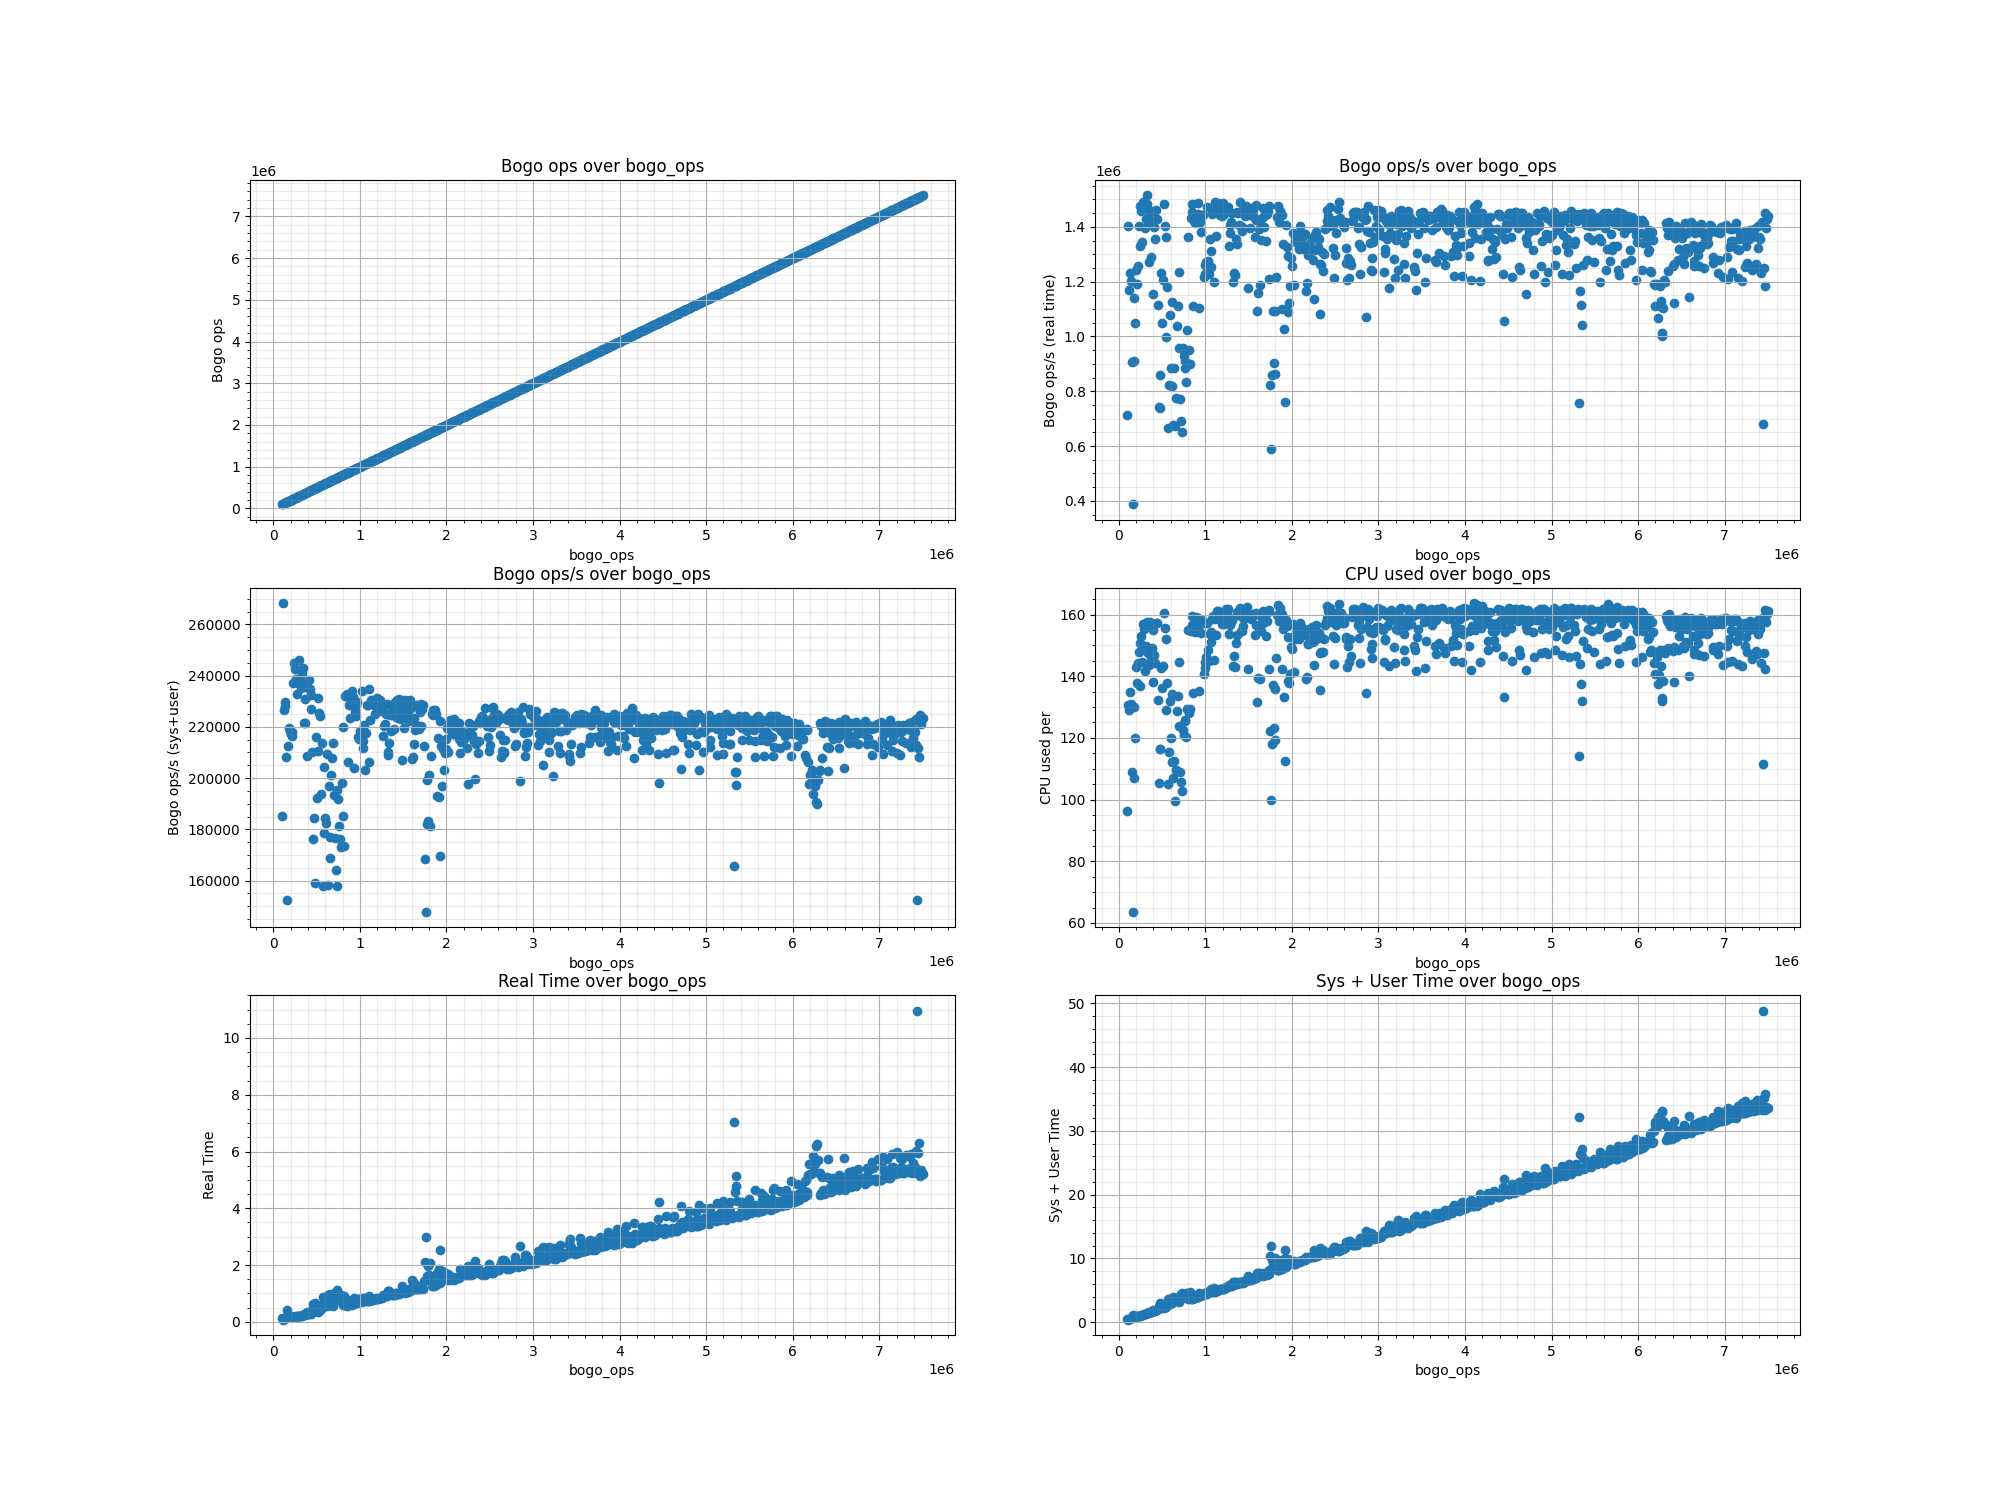
\includegraphics[width=\textwidth]{./pipe/image/pipe-ops-3.png}
\subsection{pipe-data-size}
\nquote{--pipe-data-size N}{specifies the size in bytes of each write to the pipe (range from 4 bytes to 4096 bytes). Setting a small data
size will cause more writes to be buffered in the pipe, hence reducing the context switch rate between the  pipe
writer and pipe reader processes. Default size is the page size.}
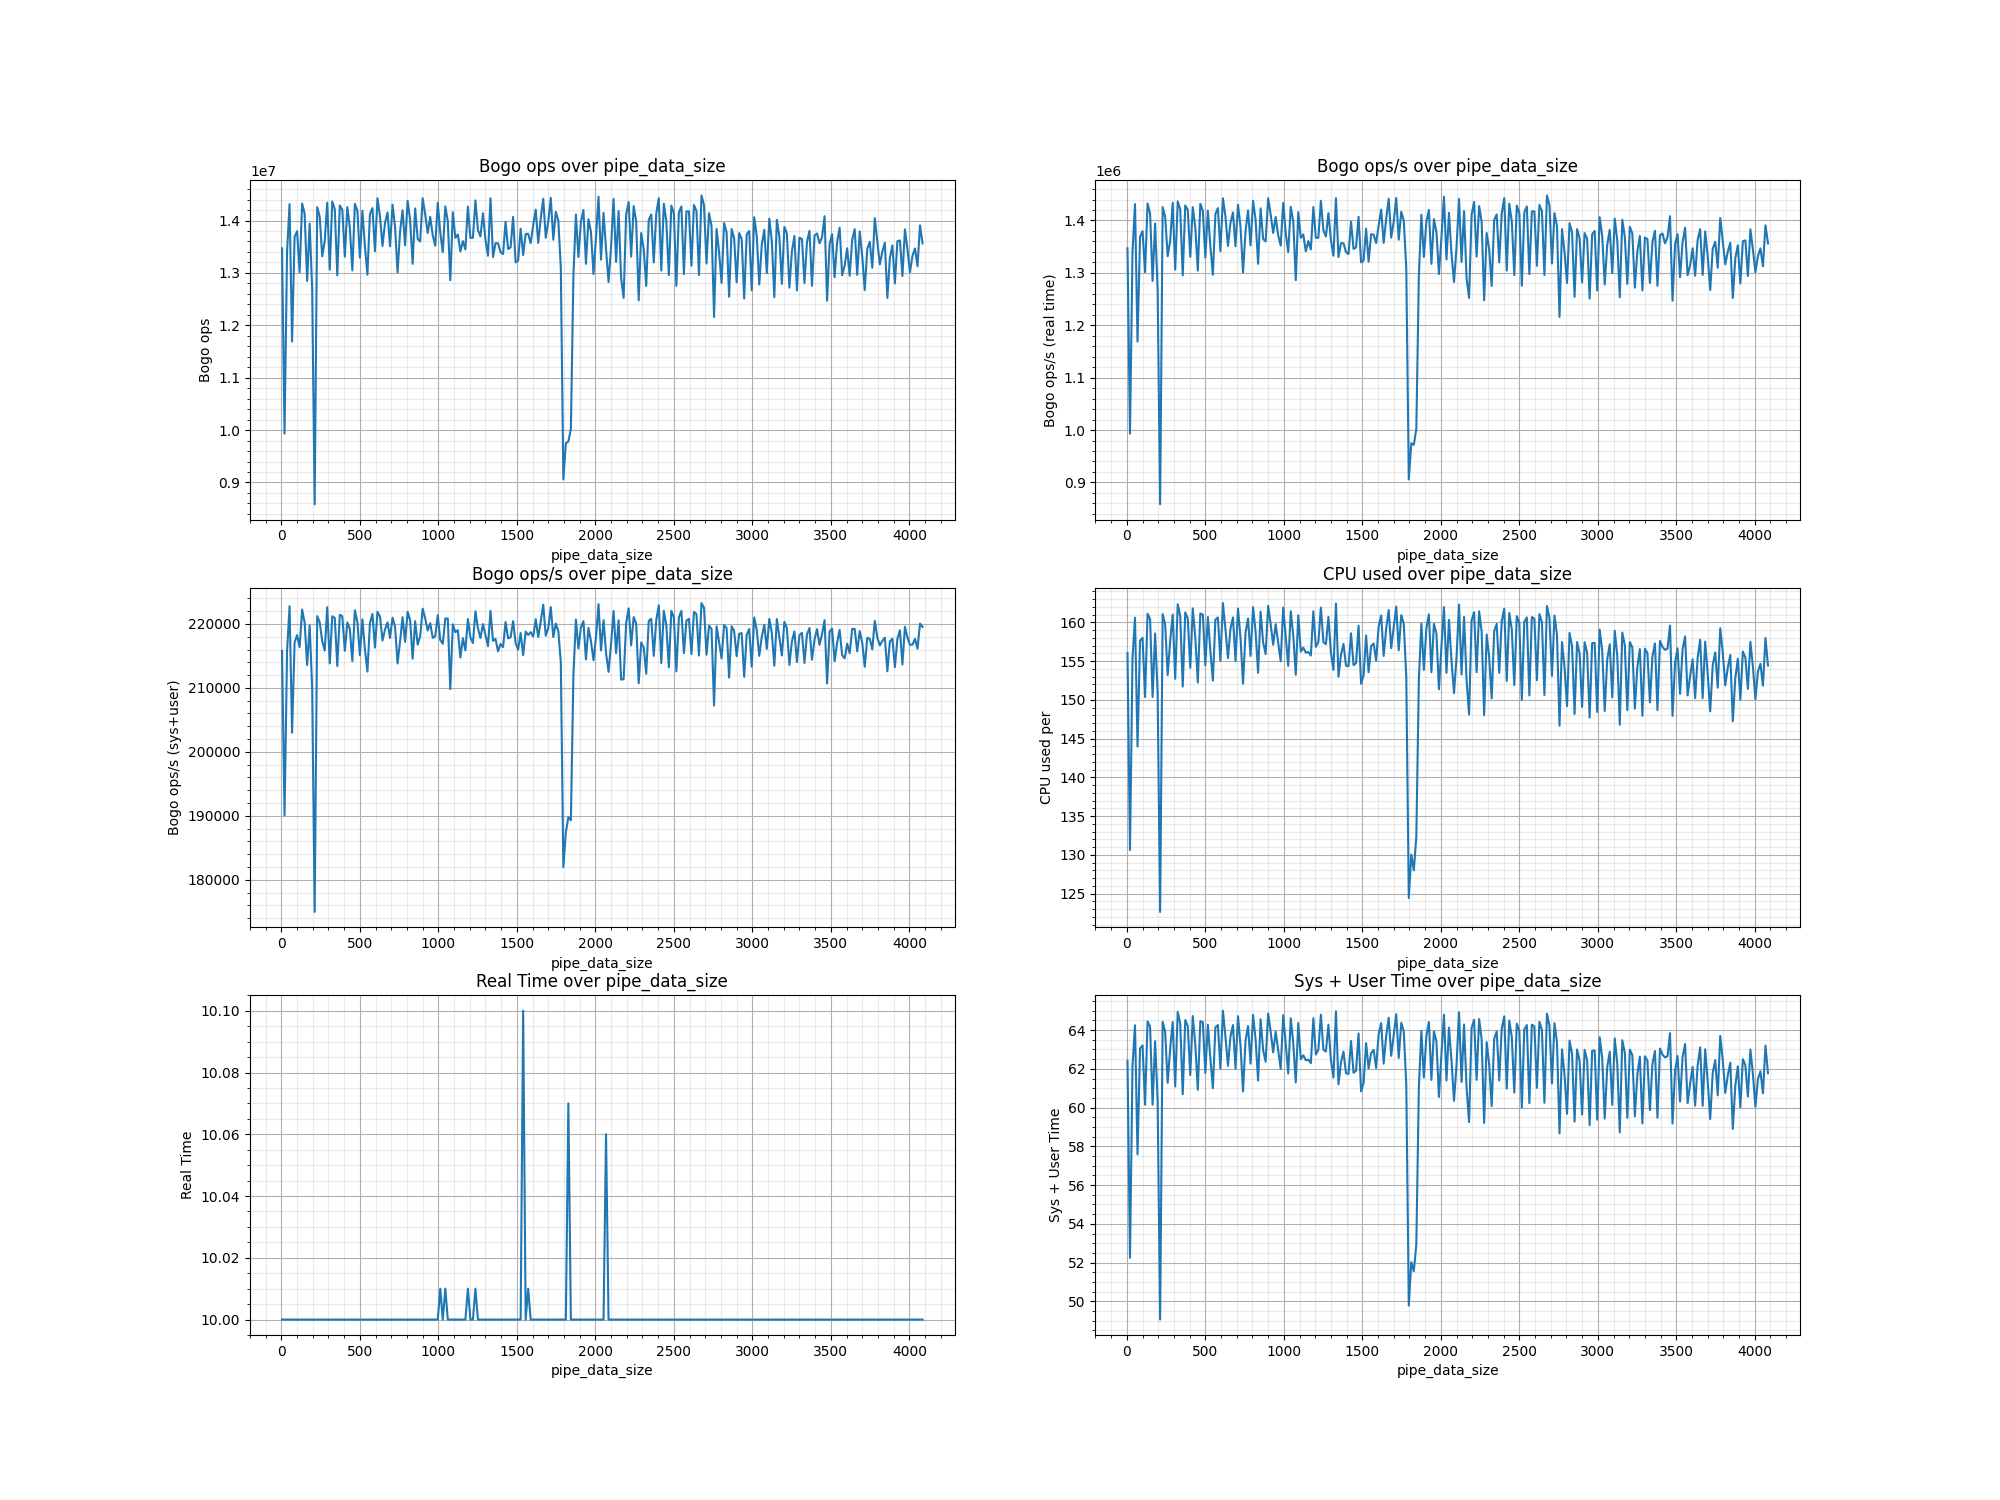
\includegraphics[width=\textwidth]{./pipe/image/pipe-data-size-bogops.png}

